\documentclass[10pt,a4paper,twocolumn]{article}

\newcommand{\projecttitle}{Supplementary material for ``Is the closing-auction imbalance already in the price?''
}

\usepackage{iftex}
\ifPDFTeX
  \usepackage[T1]{fontenc}
  \usepackage[utf8]{inputenc}
  \IfFileExists{carlito.sty}%
    {\usepackage[sfdefault]{carlito}}%
    {\usepackage[scaled=0.92]{helvet}\renewcommand{\familydefault}{\sfdefault}}%
  \usepackage{courier}
\else
  \usepackage[no-math]{fontspec}
  \setmainfont{Carlito}[Extension=.ttf, UprightFont=*-Regular, BoldFont=*-Bold,
    ItalicFont=*-Italic, BoldItalicFont=*-BoldItalic]
\fi

\usepackage[margin=18mm,bottom=20mm,columnsep=7mm]{geometry}
\usepackage{amsmath}
\usepackage{xcolor}
\usepackage{graphicx}
\usepackage{tabularx}
\usepackage{array}
\usepackage{booktabs}
\usepackage{enumitem}
\usepackage{titlesec}
\usepackage{needspace}
\usepackage[font=small,labelfont=bf]{caption}
\usepackage[hidelinks]{hyperref}
\hypersetup{pdftitle={\projecttitle},
            pdfsubject={CSE558 Data Science, Monsoon 2026: Midterm Project Report}}

\titleformat{\section}{\normalfont\large\bfseries}{\thesection.}{0.5em}{}
\titlespacing*{\section}{0pt}{12pt}{3pt}
\titleformat{\subsection}{\normalfont\normalsize\bfseries}{\thesubsection}{0.5em}{}
\titlespacing*{\subsection}{0pt}{10pt}{2pt}
\newcommand{\sectionbreak}{\needspace{10\baselineskip}}
\newcommand{\subsectionbreak}{\needspace{10\baselineskip}}

\setlength{\parindent}{0pt}
\setlength{\parskip}{4pt}
\setlist{leftmargin=1.2em, itemsep=2pt, topsep=2pt, parsep=0pt}
\renewcommand{\arraystretch}{1.25}
\setlength{\tabcolsep}{4pt}
\newcolumntype{L}[1]{>{\raggedright\arraybackslash}p{#1}}
\newcolumntype{Y}{>{\raggedright\arraybackslash}X}
\newcolumntype{K}[1]{>{\raggedright\arraybackslash\bfseries\boldmath}p{#1}}

\newcommand{\field}[2]{\textbf{#1}~#2\par}
\newcommand{\tpart}[2]{\par\needspace{12\baselineskip}\smallskip\textbf{#1)~#2}\par}
\newcommand{\minihead}[1]{\par\needspace{8\baselineskip}\smallskip\textbf{#1}\par}
\newcommand{\code}[1]{\texttt{#1}}

\graphicspath{{../figures/}}
\newcommand{\nRawRows}{5{,}237{,}980}
\newcommand{\nRawCols}{17}
\newcommand{\nRawCells}{89{,}045{,}660}
\newcommand{\nCleanRows}{5{,}237{,}760}
\newcommand{\nEncCols}{223}
\newcommand{\nEncCells}{1{,}168{,}020{,}480}
\newcommand{\nEncNumeric}{13}
\newcommand{\nEncEngineered}{5}
\newcommand{\nStocks}{200}
\newcommand{\nDays}{481}
\newcommand{\nMemBefore}{934}
\newcommand{\nMemAfter}{400}
\newcommand{\nMissingBefore}{5{,}752{,}930}
\newcommand{\nMissingAfter}{5{,}751{,}289}
\newcommand{\nEmptyRows}{220}
\newcommand{\nStructuralRows}{2{,}856{,}960}
\newcommand{\nFarOutliers}{207}
\newcommand{\nWinsorRows}{10{,}475}
\newcommand{\nWinsorLow}{-49.4}
\newcommand{\nWinsorHigh}{51.8}
\newcommand{\nFenceIqr}{32.5\%}
\newcommand{\nFenceIqrThree}{25.8\%}
\newcommand{\nFenceMad}{25.0\%}
\newcommand{\nFenceSigma}{0.12\%}
\newcommand{\nFenceCheb}{0.009\%}
\newcommand{\nStockDaysPresent}{95{,}232}
\newcommand{\nStockDaysMissing}{968}
\newcommand{\nStocksWithGaps}{15}
\newcommand{\nMaxMissingDays}{295}
\newcommand{\nIndexUnexplained}{$2.1\times10^{-8}$}
\newcommand{\nIndexWeightSum}{1.0000}
\newcommand{\nIndexWeightMax}{0.040}
\newcommand{\nIndexResidSd}{0.005}
\newcommand{\nTargetSd}{9.5}
\newcommand{\nTargetKurt}{22.6}
\newcommand{\nTargetSkew}{0.20}
\newcommand{\nSpreadMedian}{3.69}
\newcommand{\nTailObserved}{1.49\%}
\newcommand{\nTailNormal}{0.27\%}
\newcommand{\nTailCheb}{11.1\%}
\newcommand{\nTailRatio}{5.5}
\newcommand{\nEmptyNoTarget}{88}
\newcommand{\nStockDaysBefore}{95{,}236}
\newcommand{\nStructuralCells}{5{,}713{,}920}
\newcommand{\nFarPostMissing}{37{,}162}
\newcommand{\nGofChi}{98{,}064}
\newcommand{\nGofDf}{17}
\newcommand{\nAcfOne}{0.78}
\newcommand{\nAcfFive}{0.11}
\newcommand{\nAcfSix}{-0.06}
\newcommand{\nFlagSell}{40\%}
\newcommand{\nFlagBuy}{39\%}
\newcommand{\nFlagNone}{22\%}
\newcommand{\nBalancedPre}{13\%}
\newcommand{\nBalancedPost}{25\%}
\newcommand{\nSdm}{1.85}
\newcommand{\nTestRows}{952{,}320}
\newcommand{\nOneEst}{0.47}
\newcommand{\nOneCi}{0.44 to 0.49}
\newcommand{\nOneT}{32.5}
\newcommand{\nOneDf}{480}
\newcommand{\nOneP}{$8.0\times10^{-124}$}
\newcommand{\nOneRawEst}{0.48}
\newcommand{\nOneRawCi}{0.45 to 0.51}
\newcommand{\nOneBootCi}{0.44 to 0.49}
\newcommand{\nOneNaiveZ}{42.0}
\newcommand{\nOneNaiveN}{738{,}083}
\newcommand{\nOneOverlapN}{4{,}106{,}317}
\newcommand{\nOneWelchT}{41.9}
\newcommand{\nOneWelchDiff}{0.93}
\newcommand{\nOneVarRatio}{1.09}
\newcommand{\nOnePositiveDays}{458}
\newcommand{\nOneShareOfSdm}{27\%}
\newcommand{\nTwoChi}{33.2}
\newcommand{\nTwoDf}{2}
\newcommand{\nTwoP}{$6.1\times10^{-8}$}
\newcommand{\nTwoN}{95{,}193}
\newcommand{\nTwoV}{0.019}
\newcommand{\nTwoVThreshold}{0.10}
\newcommand{\nTwoMinExpected}{6{,}020}
\newcommand{\nTwoUpBuy}{50.4\%}
\newcommand{\nTwoUpSell}{48.4\%}
\newcommand{\nTwoDiff}{2.0}
\newcommand{\nTwoDiffCi}{1.3 to 2.7}
\newcommand{\nTwoPropZ}{5.73}
\newcommand{\nTwoG}{33.2}
\newcommand{\nTwoDayT}{3.62}
\newcommand{\nTwoDayP}{$1.6\times10^{-4}$}
\newcommand{\nTwoAllChi}{1{,}233}
\newcommand{\nTwoAllN}{951{,}770}
\newcommand{\nThreeEst}{0.047}
\newcommand{\nThreeCi}{0.040 to 0.054}
\newcommand{\nThreeT}{13.6}
\newcommand{\nThreeDf}{480}
\newcommand{\nThreeP}{$7.8\times10^{-36}$}
\newcommand{\nThreeThreshold}{0.02}
\newcommand{\nThreePre}{0.032}
\newcommand{\nThreePreCi}{0.028 to 0.037}
\newcommand{\nThreePost}{0.080}
\newcommand{\nThreePostCi}{0.076 to 0.084}
\newcommand{\nThreeRatio}{2.5}
\newcommand{\nThreeFisherZ}{20.5}
\newcommand{\nThreeSignDays}{363}
\newcommand{\nThreeSignP}{$4.8\times10^{-30}$}
\newcommand{\nThreeWilcoxonP}{$2.2\times10^{-33}$}
\newcommand{\nThreePooledPre}{0.030}
\newcommand{\nThreePooledPost}{0.072}
\newcommand{\nThreePooledPreT}{20.8}
\newcommand{\nThreePooledPostT}{49.8}
\newcommand{\nFourF}{0.771}
\newcommand{\nFourCi}{0.766 to 0.775}
\newcommand{\nFourDf}{476{,}159}
\newcommand{\nFourP}{$<10^{-300}$}
\newcommand{\nFourSdPre}{10.5}
\newcommand{\nFourSdPost}{9.2}
\newcommand{\nFourKurtPre}{21}
\newcommand{\nFourKurtPost}{24}
\newcommand{\nFourBf}{3{,}954}
\newcommand{\nFourBfP}{$<10^{-300}$}
\newcommand{\nFourDayRatio}{0.79}
\newcommand{\nFourDayRatioCi}{0.77 to 0.80}
\newcommand{\nFourDayT}{-24.5}
\newcommand{\nFourWinsF}{0.779}
\newcommand{\nFourLow}{0.90}
\newcommand{\nFourHigh}{1.11}
\newcommand{\nFourDrop}{23\%}
\newcommand{\nFiveN}{738{,}083}
\newcommand{\nFiveEst}{39.2\%}
\newcommand{\nFiveCi}{39.1 to 39.3}
\newcommand{\nFiveZ}{-185.4}
\newcommand{\nFiveP}{$1.000$}
\newcommand{\nFiveGross}{52.0\%}
\newcommand{\nFiveNet}{-2.40}
\newcommand{\nFiveThreshold}{52\%}
\newcommand{\nFiveDayT}{-133.0}
\newcommand{\nBoundT}{0.028}
\newcommand{\nBoundCheb}{0.064}
\newcommand{\nBoundHoeff}{6.42}
\newcommand{\nBoundChebRatio}{2.3}
\newcommand{\nBoundHoeffRatio}{228}
\newcommand{\nBoundTCi}{0.44 to 0.49}
\newcommand{\nBoundChebCi}{0.40 to 0.53}
\newcommand{\nBoundHoeffCi}{-6.0 to 6.9}
\newcommand{\nBoundRange}{51.8}
\newcommand{\nJumpReal}{0.057}
\newcommand{\nJumpRealCi}{0.040 to 0.074}
\newcommand{\nJumpLast}{0.193}
\newcommand{\nJumpLastCi}{0.181 to 0.206}
\newcommand{\nJumpFour}{0.084}
\newcommand{\nJumpTwo}{0.054}
\newcommand{\nJumpSevenMin}{-0.082}
\newcommand{\nIcBeforeBoundary}{-0.037}
\newcommand{\nIcAtBoundary}{0.108}
\newcommand{\nIcLast}{0.247}
\newcommand{\nIcMin}{-0.064}
\newcommand{\nSensWith}{0.054}
\newcommand{\nSensWithCi}{0.047 to 0.060}
\newcommand{\nSensWithout}{0.014}
\newcommand{\nSensWithoutCi}{0.006 to 0.021}
\newcommand{\nRobPositive}{11}
\newcommand{\nRobTotal}{11}
\newcommand{\nPermOneP}{$5.0\times10^{-4}$}
\newcommand{\nPermOneMax}{0.039}
\newcommand{\nPermOneN}{2{,}000}
\newcommand{\nFlipThreeP}{$1.0\times10^{-4}$}
\newcommand{\nFlipThreeMax}{0.014}
\newcommand{\nFlipThreeN}{10{,}000}
\newcommand{\nFinalGross}{2.40}
\newcommand{\nFinalHalf}{1.92}
\newcommand{\nFinalNet}{0.48}
\newcommand{\nFinalNetCi}{0.39 to 0.58}
\newcommand{\nFinalT}{9.7}
\newcommand{\nFinalHit}{52.7\%}
\newcommand{\nFinalFirst}{0.74}
\newcommand{\nFinalSecond}{0.23}
\newcommand{\nFinalSecondCi}{0.10 to 0.36}
\newcommand{\nStrongGross}{1.77}
\newcommand{\nStrongHalf}{3.81}
\newcommand{\nStrongNet}{-1.99}
\newcommand{\nStrongNetCi}{-2.18 to -1.79}
\newcommand{\nBreakPre}{0.30}
\newcommand{\nBreakPost}{0.71}
\newcommand{\nTFitDf}{3.1}
\newcommand{\nTFitScale}{6.2}
\newcommand{\nTFitChi}{568}
\newcommand{\nTFitGain}{0.125}
\newcommand{\nNormChi}{98{,}064}
\newcommand{\nFlipMean}{2.69}
\newcommand{\nFlipVar}{6.59}
\newcommand{\nFlipDispersion}{2.45}
\newcommand{\nFlipZero}{19.6\%}
\newcommand{\nFlipZeroPoisson}{6.8\%}
\newcommand{\nFlipChi}{189{,}527}
\newcommand{\nFlipDf}{10}
\newcommand{\nMidOneEst}{0.31}
\newcommand{\nMidOneCi}{0.28 to 0.35}
\newcommand{\nMidOneT}{19.7}
\newcommand{\nWapOneEst}{0.31}
\newcommand{\nMidOneRetained}{101\%}
\newcommand{\nMidFiveHit}{37.3\%}
\newcommand{\nWapFiveHit}{38.0\%}
\newcommand{\nCmItems}{95{,}232}
\newcommand{\nCmCounters}{14{,}000}
\newcommand{\nCmWidth}{2{,}000}
\newcommand{\nCmDepth}{7}
\newcommand{\nCmWithin}{100\%}
\newcommand{\nCmMaxShare}{66\%}
\newcommand{\nCmTop}{9}
\newcommand{\nCmMemory}{15\%}
\newcommand{\nMdeOne}{0.036}
\newcommand{\nDaysOne}{1}
\newcommand{\nThrOne}{1.85}
\newcommand{\nMdeThree}{0.010}
\newcommand{\nDaysThree}{115}
\newcommand{\nThrThree}{0.02}
\newcommand{\nMdeFour}{0.027}
\newcommand{\nDaysFour}{32}
\newcommand{\nThrFour}{0.105}
\newcommand{\nMdeFive}{0.002}
\newcommand{\nDaysFive}{5}
\newcommand{\nThrFive}{0.02}
\newcommand{\nMdeOneRatio}{52}
\newcommand{\nRobRows}{first half of days & 0.024 & 0.087 & +0.063 (0.054 to 0.072) \\
second half of days & 0.041 & 0.073 & +0.031 (0.022 to 0.041) \\
size: low & 0.050 & 0.080 & +0.029 (0.021 to 0.037) \\
size: mid & 0.033 & 0.075 & +0.041 (0.032 to 0.051) \\
size: high & 0.016 & 0.098 & +0.081 (0.071 to 0.091) \\
spread: low & 0.016 & 0.094 & +0.078 (0.069 to 0.088) \\
spread: mid & 0.035 & 0.073 & +0.038 (0.028 to 0.047) \\
spread: high & 0.046 & 0.082 & +0.036 (0.028 to 0.043) \\
day volatility: low & 0.038 & 0.077 & +0.039 (0.029 to 0.050) \\
day volatility: mid & 0.032 & 0.080 & +0.048 (0.036 to 0.059) \\
day volatility: high & 0.028 & 0.082 & +0.055 (0.041 to 0.068) \\}
\newcommand{\nJumpRows}{15:50:00 to 15:51:00 & -0.019 & -0.032 to -0.006 \\
15:51:00 to 15:52:00 & +0.054 & 0.043 to 0.066 \\
15:52:00 to 15:53:00 & +0.010 & -0.002 to 0.022 \\
15:53:00 to 15:54:00 & -0.006 & -0.019 to 0.007 \\
15:54:00 to 15:55:00 & +0.057 & 0.040 to 0.074 \\
15:55:00 to 15:56:00 & -0.056 & -0.071 to -0.041 \\
15:56:00 to 15:57:00 & -0.082 & -0.094 to -0.070 \\
15:57:00 to 15:58:00 & +0.084 & 0.073 to 0.096 \\
15:58:00 to 15:59:00 & +0.193 & 0.181 to 0.206 \\}
\newcommand{\nSixEst}{0.140}
\newcommand{\nSixCi}{0.134 to 0.146}
\newcommand{\nSixT}{46.9}
\newcommand{\nSixDf}{179}
\newcommand{\nSixP}{$8.4\times10^{-103}$}
\newcommand{\nSixPerm}{$1.0\times10^{-4}$}
\newcommand{\nSixThreshold}{0.01}
\newcommand{\nSixMlp}{0.192}
\newcommand{\nSixBase}{0.052}
\newcommand{\nSixRatio}{3.7}
\newcommand{\nSixTestDays}{180}
\newcommand{\nSixTrainRows}{2{,}600{,}950}
\newcommand{\nSixTestRows}{359{,}960}
\newcommand{\nSixFeatures}{19}
\newcommand{\nLgbmIc}{0.200}
\newcommand{\nLgbmGain}{0.148}
\newcommand{\nLgbmGainCi}{0.142 to 0.153}
\newcommand{\nMlpLgbm}{-0.008}
\newcommand{\nMlpLgbmCi}{-0.009 to -0.006}
\newcommand{\nGruIc}{0.195}
\newcommand{\nSnapIc}{0.172}
\newcommand{\nGruGain}{0.022}
\newcommand{\nGruGainCi}{0.020 to 0.025}
\newcommand{\nDmZeroT}{17.1}
\newcommand{\nDmLinT}{16.9}
\newcommand{\nDmLinP}{$2.4\times10^{-39}$}
\newcommand{\nSeedSdMlp}{0.0010}
\newcommand{\nSeedSdLgbm}{0.0004}
\newcommand{\nSeedSdGru}{0.0022}
\newcommand{\nSeedRatio}{145}
\newcommand{\nMidGain}{-0.010}
\newcommand{\nMidGainCi}{-0.016 to -0.003}
\newcommand{\nMidMlp}{0.031}
\newcommand{\nMidBase}{0.040}
\newcommand{\nMidShare}{-7\%}
\newcommand{\nSelNet}{0.68}
\newcommand{\nSelNetCi}{0.58 to 0.77}
\newcommand{\nSelT}{13.6}
\newcommand{\nSelHit}{53.5\%}
\newcommand{\nSelShare}{13.5\%}
\newcommand{\nSelTrades}{48{,}534}
\newcommand{\nSelMidNet}{-0.40}
\newcommand{\nSelMidNetCi}{-0.51 to -0.28}
\newcommand{\nSelMidHit}{46.8\%}
\newcommand{\nSelMidT}{-6.9}
\newcommand{\nSelMidP}{$1.000$}
\newcommand{\nCtAcc}{82.3\%}
\newcommand{\nCtZ}{388}
\newcommand{\nCtN}{359{,}960}
\newcommand{\nCtDayCi}{82.0 to 82.7}
\newcommand{\nImpFirst}{depth imbalance}
\newcommand{\nImpFirstShare}{19\%}
\newcommand{\nImpSecond}{spread bps}
\newcommand{\nImpThird}{ref gap bps}
\newcommand{\nImpImbShare}{5\%}
\newcommand{\nHolmOne}{$4.0\times10^{-123}$}
\newcommand{\nHolmTwo}{$1.2\times10^{-7}$}
\newcommand{\nHolmThree}{$2.3\times10^{-35}$}
\newcommand{\nHolmFour}{$<10^{-300}$}
\newcommand{\nHolmFive}{$1.000$}
\newcommand{\nHolmSix}{$3.4\times10^{-102}$}


\begin{document}

\twocolumn[%
{\small\bfseries CSE558 Data Science\ \ \textbullet\ \ Midterm Project Report\ \ \textbullet\ \ Supplementary material\par}
\vspace{4pt}
{\LARGE\bfseries\raggedright\projecttitle\par}
\vspace{6pt}
\rule{\linewidth}{1pt}
{\small This supplement adds the figures and tables behind every check in the main report. Every number is generated
by the same code run as the main report. Section numbers here are prefixed with S.\par}
\vspace{10pt}
]

\renewcommand{\thesection}{S\arabic{section}}
\renewcommand{\thefigure}{S\arabic{figure}}
\renewcommand{\thetable}{S\arabic{table}}

\section{Data processing}

\minihead{The hidden index}
The target is a stock's 60\,s WAP return minus an index's 60\,s return, and the index is not given. At every
timestamp the implied index return (stock return minus target) is the same for all stocks to within \nIndexResidSd{}
bps, so it is one series. Regressing it on the 200 stock returns recovers positive weights that sum to
\nIndexWeightSum{} and leave unexplained variance \nIndexUnexplained. The weights come in a few discrete tiers
(Figure~\ref{fig:sweights}), the largest at \nIndexWeightMax.

\begin{figure}[!ht]
  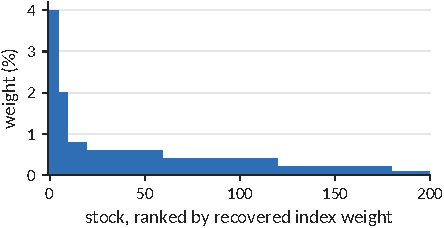
\includegraphics[width=\linewidth]{figS_index_weights}
  \caption{The hidden index is a tiered weighted average of the 200 stocks. Bars are the recovered weights, largest
  first.}
  \label{fig:sweights}
\end{figure}

\begin{figure*}[!t]
  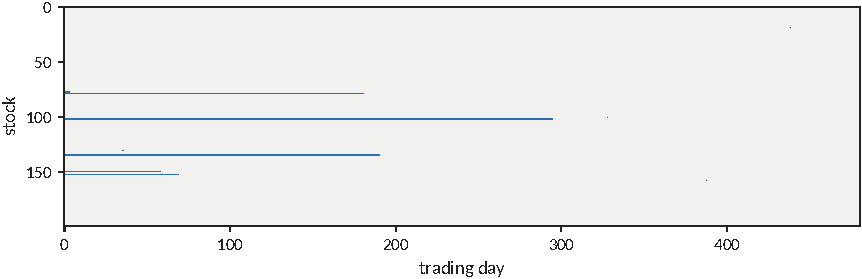
\includegraphics[width=\linewidth]{figS_coverage}
  \caption{Panel coverage: each row is a stock, each column a trading day, and blue marks a stock-day with no data.
  \nStockDaysMissing{} of 96{,}200 stock-days are absent, almost all from \nStocksWithGaps{} stocks that join the
  panel late; one stock is missing for \nMaxMissingDays{} days. Every comparison in the report is made within a day.}
  \label{fig:scoverage}
\end{figure*}

\minihead{Streaming summary}
A Count-Min sketch with \nCmDepth{} rows of \nCmWidth{} counters ($\varepsilon=0.001$, $\delta=0.01$, universal
hashing modulo the prime $2^{31}-1$) totalled the imbalance shares of \nCmItems{} stock-days in one pass. It uses
\nCmCounters{} counters, \nCmMemory{} of exact counting. The guarantee says each estimate exceeds the truth by at most
$\varepsilon N$ with probability at least $1-\delta$; here \nCmWithin{} of estimates do, the worst at \nCmMaxShare{} of
the bound (Figure~\ref{fig:scm}).

\begin{figure}[!ht]
  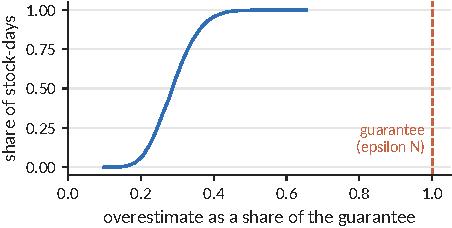
\includegraphics[width=\linewidth]{figS_countmin}
  \caption{Every Count-Min estimate stays inside its guarantee. The curve is the cumulative share of stock-days whose
  overestimate is below a given fraction of $\varepsilon N$.}
  \label{fig:scm}
\end{figure}

\section{Distributions}

\begin{figure}[!ht]
  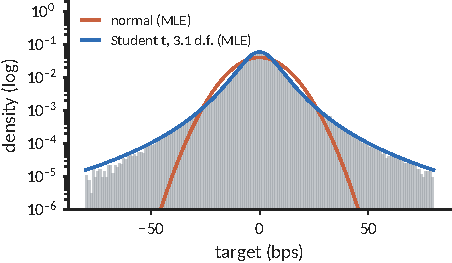
\includegraphics[width=\linewidth]{figS_tfit}
  \caption{A Student $t$ with \nTFitDf{} degrees of freedom fits the tails that a normal misses. Both curves are
  maximum-likelihood fits to the minute snapshots; grey is the histogram.}
  \label{fig:stfit}
\end{figure}

The $t$ fit raises the log-likelihood by \nTFitGain{} per row and cuts the 20-bin $\chi^2$ goodness-of-fit statistic
from \nNormChi{} to \nTFitChi. With fewer than four degrees of freedom the fourth moment is infinite, which is why the
sample kurtosis (\nTargetKurt) is unstable and why our tests rely on day averages.

\begin{figure}[!ht]
  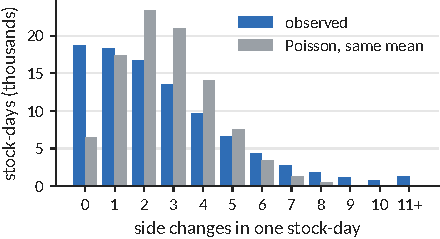
\includegraphics[width=\linewidth]{figS_flips}
  \caption{Auctions either hold one side all along or churn: far more stock-days have no side change, and more have
  many, than a Poisson count with the same mean allows.}
  \label{fig:sflips}
\end{figure}

A stock changes imbalance side \nFlipMean{} times per auction on average, with variance \nFlipVar. A Poisson has
variance equal to its mean, so the dispersion of \nFlipDispersion{} rejects it ($\chi^2=\nFlipChi$ on \nFlipDf{}
d.f.).

\section{P2: learned models}

{\footnotesize
\begin{tabularx}{\linewidth}{@{}L{1.7cm} Y@{}}
\toprule
\textbf{Setting} & \textbf{Value, fixed before training} \\
\midrule
Split & train days 0 to 240 (\nSixTrainRows{} rows), early stopping on 241 to 300, test on 301 to 480 \\
Features & signed imbalance, $|$imbalance$|$/matched, side, log matched size, spread, near and far gaps with
missing flags, reference-to-WAP gap, depth imbalance, time, phase, WAP returns over 10, 30, 60\,s, imbalance changes
over 10, 60\,s; no stock identity \\
MLP & 128 and 64 ReLU units, dropout 0.1, Adam at $10^{-3}$, batch 4{,}096, MSE on the winsorised target, early
stopping on validation IC \\
LightGBM & 63 leaves, learning rate 0.05, early stopping after 100 rounds \\
GRU & one layer of 64 units over the auction so far, snapshot features only \\
Seeds & 5 per model; predictions averaged \\
\bottomrule
\end{tabularx}}

{\footnotesize
\begin{tabularx}{\linewidth}{@{}L{3.3cm} Y@{}}
\toprule
\textbf{Comparison (held-out days)} & \textbf{Estimate (95\% CI)} \\
\midrule
MLP minus imbalance, WAP target & $+\nSixEst$ (\nSixCi) \\
LightGBM minus imbalance & $+\nLgbmGain$ (\nLgbmGainCi) \\
MLP minus LightGBM & \nMlpLgbm{} (\nMlpLgbmCi) \\
GRU minus snapshot-only MLP & $+\nGruGain$ (\nGruGainCi) \\
MLP minus imbalance, mid target & \nMidGain{} (\nMidGainCi) \\
Diebold-Mariano, MLP vs zero & $t=\nDmZeroT$ \\
Diebold-Mariano, MLP vs linear & $t=\nDmLinT$ \\
Seed SD of mean IC (MLP, LGBM, GRU) & \nSeedSdMlp, \nSeedSdLgbm, \nSeedSdGru \\
\bottomrule
\end{tabularx}}

The GRU's gain over the snapshot-only MLP says the path of the auction carries information beyond its current state,
on the WAP target. Seed-to-seed variation is two orders of magnitude below every gain (Figure~\ref{fig:sseeds}), so
none of these differences is training noise.

\begin{figure}[!ht]
  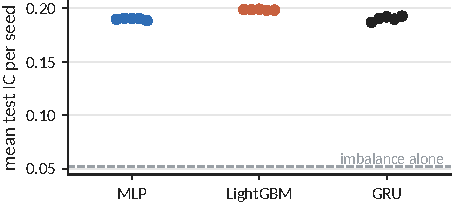
\includegraphics[width=\linewidth]{figS_seeds}
  \caption{Five seeds per model agree almost exactly, far above the imbalance alone on the WAP target.}
  \label{fig:sseeds}
\end{figure}

\begin{figure}[!ht]
  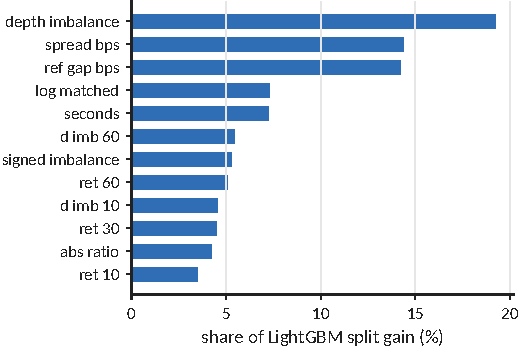
\includegraphics[width=\linewidth]{figS_importance}
  \caption{The models lean on book depth and the spread, the inputs that move the WAP mechanically, more than on the
  imbalance (\nImpImbShare{} of split gain).}
  \label{fig:simportance}
\end{figure}

\section{P3: placebo, subgroups and the classifier test}

\begin{figure}[!ht]
  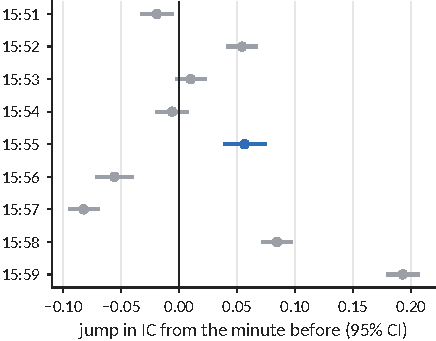
\includegraphics[width=\linewidth]{figS_placebo}
  \caption{The jump at 15:55 is real but not unique: the last minute jumps more. Each line is the change in IC from
  the previous minute, with a 95\% interval over days.}
  \label{fig:splacebo}
\end{figure}

\begin{figure}[!ht]
  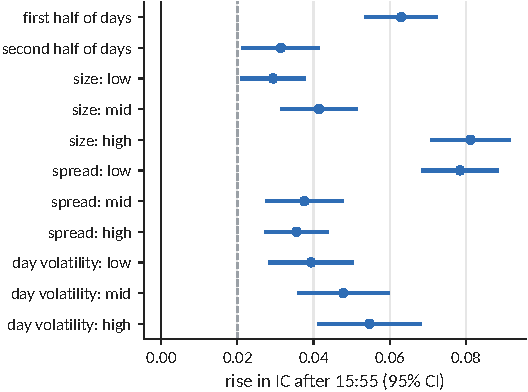
\includegraphics[width=\linewidth]{figS_robustness}
  \caption{The post-15:55 rise holds in every subgroup fixed in advance. Dashed line: the 0.02 threshold.}
  \label{fig:srob}
\end{figure}

{\footnotesize
\begin{tabularx}{\linewidth}{@{}L{2.6cm} L{0.9cm} L{0.9cm} Y@{}}
\toprule
\textbf{Subgroup} & \textbf{IC pre} & \textbf{IC post} & \textbf{$\Delta$IC (95\% CI)} \\
\midrule
\nRobRows
\bottomrule
\end{tabularx}}

\begin{figure}[!ht]
  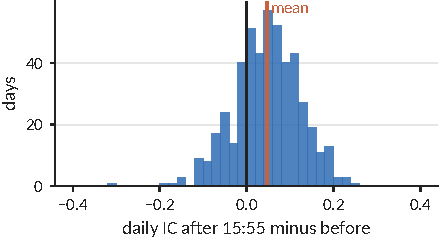
\includegraphics[width=\linewidth]{fig_daily_ic}
  \caption{Day by day, the imbalance predicts better after 15:55 on \nThreeSignDays{} of \nDays{} days.}
  \label{fig:sdaily}
\end{figure}

\minihead{Classifier two-sample test}
If the auction state did not change at 15:55, no classifier could tell pre from post snapshots better than chance.
LightGBM, trained without the features that are missing by rule, is right on \nCtAcc{} of \nCtN{} held-out snapshots
($z=\nCtZ$; day-level 95\% CI \nCtDayCi\%). This is the lecture 6 one-proportion z-test applied to a learned
classifier's accuracy.

\section{P4: edge, cost and the learned rule}

\begin{figure}[!ht]
  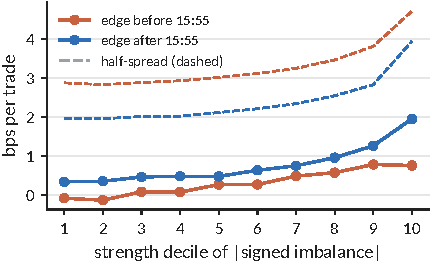
\includegraphics[width=\linewidth]{figS_edge_strength}
  \caption{Stronger imbalances earn more, but their stocks quote wider spreads, so the edge never catches the cost.
  Solid: gross edge by strength decile; dashed: the same stocks' half-spread.}
  \label{fig:sstrength}
\end{figure}

{\footnotesize
\begin{tabularx}{\linewidth}{@{}L{3.3cm} Y@{}}
\toprule
\textbf{Rule (held-out days)} & \textbf{Net bps per trade (95\% CI)} \\
\midrule
MLP signal above half-spread, WAP target & $+\nSelNet$ (\nSelNetCi), hit rate \nSelHit \\
Same rule, mid-price target & \nSelMidNet{} (\nSelMidNetCi), hit rate \nSelMidHit \\
Imbalance, 15:59 snapshot only & $+\nFinalNet$ (\nFinalNetCi) \\
\quad first half of days & $+\nFinalFirst$ \\
\quad second half of days & $+\nFinalSecond$ (\nFinalSecondCi) \\
\bottomrule
\end{tabularx}}

\section{Power}

{\footnotesize
\begin{tabularx}{\linewidth}{@{}L{1.0cm} L{2.4cm} L{1.4cm} Y@{}}
\toprule
\textbf{Test} & \textbf{Detectable at 80\%} & \textbf{Threshold} & \textbf{Days needed at threshold} \\
\midrule
Test 1 & \nMdeOne{} bps & \nThrOne{} bps & \nDaysOne \\
Test 4 & \nMdeThree{} IC & \nThrThree{} IC & \nDaysThree \\
Test 5 & \nMdeFour{} log ratio & \nThrFour & \nDaysFour \\
Test 6 & \nMdeFive{} hit rate & \nThrFive & \nDaysFive \\
\bottomrule
\end{tabularx}}

\begin{figure}[!ht]
  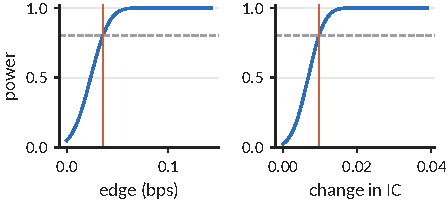
\includegraphics[width=\linewidth]{figS_power}
  \caption{With 481 days, power reaches 80\% (dashed) at effects far below our thresholds. Left: Test 1; right:
  Test 4. The vertical line marks the detectable effect.}
  \label{fig:spower}
\end{figure}

\section{Pre-registration record}

Every threshold was written down, with a date, before the analysis it governs was run. Changes made before any test
ran, and results that missed their pre-set criterion, are listed here.

{\footnotesize
\begin{tabularx}{\linewidth}{@{}L{1.4cm} Y@{}}
\toprule
\textbf{When} & \textbf{What was fixed or changed} \\
\midrule
Before tests & sampling at whole minutes; the SDM as the median half-spread; Tests 1, 2, 4, 5, 6 with their
thresholds \\
Before tests & a far-price fence changed from Tukey (flags 26\%) to Chebyshev (flags \nFarOutliers{} rows); a
cleaning step dropped as a profiling artefact \\
Before checks & subgroups, placebo, power, cost, permutation, fits and sketch criteria \\
Before training & Test 3 design, models, split and checks \\
Before 5 seeds & the mid-price check, added after a one-seed run whose numbers are not reported \\
\midrule
Miss & Test 4: we predicted IC would fall after 15:55; it rose \\
Miss & Placebo: 15:55 is not the largest jump \\
Rule fired & Test 3: most of the learned gain is WAP mechanics \\
\bottomrule
\end{tabularx}}

\section{Reproduction}
One command, \code{python run\_all.py}, rebuilds every number and figure in both documents from the raw
\code{train.csv} in about seven minutes on a laptop with a consumer GPU. Every number in the text is a macro written
by the code; none is typed by hand.

\end{document}
